\subsection{Hierarchical Clustering \label{sec:authorship_clustering_methods}}

To find clusters of authors, a possible way is to use a hierarchical clustering algorithm on a rank list.
The rank list indicate if the two documents should belong to the same cluster by order of certainty.
The hierarchical clustering regroup documents following this order.

The hardest task with this clustering scheme is to find the position in the rank list where true link become less frequent than false link.
In a the clustering context, the optimal position is unknown since the true labels are not available.
The position should minimized the true links under it and the false links above it.

In this study, finding this position will also be refered as finding the \textit{cut}.
We define the true positive as true links above the cut, true negatives as false links under the cut.
In addition false positive are true links under the cut and false negatives are false links above the cut.

To find this cut, three approaches are explored : an unsupervised, a semi-supervised and a supervised.

The unsupervised method can be used when only one corpus is available and no learning procedures can be applied.

The semi-supervised learn based on a corpus with labels (training corpus) a rank list score where the cut should be for any other corpus (called testing corpus).

Finally, the supervised approach, learn based on a rank from a corpus with labels (training corpus) a model.
The model can find the optimal cut for a rank list from a new corpus (called testing corpus) generated using the same metrics as ones used for training.

\subsubsection{Algorithm and Implementation \label{sec:algorithm_and_implementation}}

The scikit-learn package~\cite{sklearn} provide an implementation bottom-up implementation of the hierarchical clustering, which is called agglomerative clustering.

The agglomerative clustering follow this procedure:
\begin{enumerate}
  \item The rank list used is converted into a 2D distances' matrix with each link representing a element of the matrix (ref. Section~\ref{sec:distances_matrix}).
  \item At the begining, each document is considered as a single document cluster.
  \item The link (element) with the lowest score in the matrix is used to merge the next clusters.
  \item The matrix is updated following a linkage criteria.
  \item 3. and 4. can be repeated until a single cluster remain.
\end{enumerate}

Multiple linkage criteria are available : \textit{Ward} (metric that aim to minimize the variance of the cluster merged), \textit{average-linkage} (use the average score of each link of the cluster merged), \textit{complete-linkage} (use the cluster merged maximal score), \textit{single-linkage} (use the cluster merged minimal score).
Example~\ref{ex:agglomerative_clustering} show an example for the merging procedures and the linkage criteria.

Ward linkage was discarded since the current implementation only allow Euclidian distance for its computation.
The merging procedure can be stopped either of the two following criteria : When a certain cluster number is reached or when the minimal score for the next merge is above a certain value.
This value is called the distance threshold.

The so called cut can be associated to the distance threshold.
The cut is a position in the rank list and the distance threshold is the score which can help to seperate the rank list.

There is one main flaw with the scikit-learn implementation.
It does not provide a way to access the current cluster at each merging step.
A possible workaround is to run the algorithm multiple time.
Each time the algorithm is stopped at a different cluster number.
This workaround introduce an overhead of $O\frac{n * (n - 1)}{2} = O(n^2)$, with $n$ equal to the number of documents.

The agglomerative clustering algorithm was reimplementated to allow access to the clusters at each steps and avoid this overhead.
The implementation profit of the generator functions that Python offers.

\begin{example}
  \small
  \centering
  \caption{Agglomerative clustering}
  \label{ex:agglomerative_clustering}

  \begin{subexample}{\linewidth}
    \centering
    \subcaption{Initial clusters and their distances}
    \begin{tabular}{c|c c c c}
      \toprule
        & A & B & C & D \\
      \midrule
      A & - & \textbf{1} & $2$ & $3$ \\
      B & - & - & $8$ & $7$\\
      C & - & - & - & $6$ \\
      D & - & - & - & - \\
      \bottomrule
    \end{tabular}
  \end{subexample}

  \vspace{0.2cm}
  The link with the smallest distance is A-B with a distance of 1.
  At the next step the clusters A and B are merged into a cluster called AB.

  \vspace{0.5cm}

  \begin{subexample}{\linewidth}
    \centering
    \subcaption{First merge using single-linkage}
    \begin{tabular}{c|c c c}
      \toprule
        & AB & C & D \\
      \midrule
      AB & - & $\text{min} \left[2, 8 \right] = 2$ & $\text{min} \left[3, 7 \right] = 3$ \\
      C  & - & - & $6$ \\
      D  & - & - & - \\
      \bottomrule
    \end{tabular}
  \end{subexample}

  \vspace{0.2cm}
  Next step will merge AB and C.

  \vspace{0.5cm}

  \begin{subexample}{\linewidth}
    \centering
    \subcaption{First merge using average-linkage}
    \begin{tabular}{c|c c c}
      \toprule
        & AB & C & D \\
      \midrule
      AB & - & $\text{avg} \left[2, 8 \right] = 5$ & $\text{avg} \left[3, 7 \right] = 4$ \\
      C  & - & - & $6$ \\
      D  & - & - & - \\
      \bottomrule
    \end{tabular}
  \end{subexample}

  \vspace{0.2cm}
  Next step will merge AB and D.

  \vspace{0.5cm}

  \begin{subexample}{\linewidth}
    \centering
    \subcaption{First merge using complete-linkage}
    \begin{tabular}{c|c c c}
      \toprule
        & AB & C & D \\
      \midrule
      AB & - & $\text{max} \left[2, 8 \right] = 8$ & $\text{max} \left[3, 7 \right] = 7$ \\
      C  & - & - & 6 \\
      D  & - & - & - \\
      \bottomrule
    \end{tabular}
  \end{subexample}

  \vspace{0.2cm}
  Next step will merge C and D.
\end{example}


\subsubsection{Parameters\label{sec:hierarchical_clustering}}

As explained in Section~\ref{sec:algorithm_and_implementation}, the hierarchical clustering decide clusters based on a bottom-up approach and have two main parameters, the stopping procedure and the linkage criterion.
The linkage criterion can be : single, complete, average linkage.
Oxquarry, Brunet, St-Jean A, St-Jean B and St-Jean copora are used for this experiment.

The goal is to understand how the linkage criterion behave for the best clustering achievable (best $B^3_{F_1}$)

The custom implementation of the hierarchical clustering is used, at each merging step, the intermediary clustering is evaluated using the $B^3_{F_1}$.
The clustering resulting in the best $B^3_{F_1}$ is kept.
This procedure is repeated for each linkage criteria and corpus / text representation.

The results are presented in Table~\ref{tab:hierarchical_clustering} and the mean for each corpus and linkage criterion.

These results can be considered as the $B^3_{F_1}$ upper bound for the clustering case using the retained rank list on these corpora.

The best linkage criterion depends on the corpus, but in average, the best $B^3_{F_1}$ is achieved with the average linkage criterion, a relative increase of 0.01 compared to the complete linkage and 0.05 compared to the single linkage.

We assumed that the better the rank list are the better the clustering is.
This assumption can be verified in Figure~\ref{fig:correlation_average_precision_b3f1}.
We can clearly observe a linear relationship between the average precision and the $B^3_{F_1}$.
The linear regression for the single linkage have a r-value of $1^{-11}$, $1^{-12}$ for the average linkage and $1^{-6}$ for the complete linkage.
This further motive this assumption.

\begin{table}
  \centering
  \caption{Best $B^3_{F_1}$ with hierarchical clustering on every rank lists and linkage criterion}
  \label{tab:hierarchical_clustering}

  \resizebox{\linewidth}{!}{
  \begin{tabular}{l l c c c}
    \toprule
    \multicolumn{2}{c}{Rank list} & \multicolumn{3}{c}{Linkage criterion} \\
    TR ID & Corpus & Single & Average & Complete \\
    \midrule
    0 & Oxquarry & 0.95 & 1.00 & 0.90 \\
    1 & Oxquarry & 0.93 & 0.93 & 0.82 \\
    2 & Oxquarry & 0.67 & 0.74 & 0.80 \\
    3 & Oxquarry & 0.77 & 0.77 & 0.84 \\
    4 & Oxquarry & 0.87 & 0.91 & 0.84 \\
    5 & Oxquarry & 0.88 & 0.89 & 0.84 \\
    6 & Oxquarry & 0.86 & 0.83 & 0.80 \\
    \midrule
    \multicolumn{2}{l}{Oxquarry mean} & 0.85 & 0.87 & 0.84 \\
    \midrule
    0 & Brunet & 0.81 & 0.82 & 0.77 \\
    1 & Brunet & 0.82 & 0.85 & 0.89 \\
    2 & Brunet & 0.77 & 0.84 & 0.77 \\
    3 & Brunet & 0.79 & 0.80 & 0.78 \\
    4 & Brunet & 0.78 & 0.82 & 0.81 \\
    5 & Brunet & 0.79 & 0.82 & 0.90 \\
    6 & Brunet & 0.86 & 0.82 & 0.87 \\
    \midrule
    \multicolumn{2}{l}{Brunet mean} & 0.80 & 0.83 & 0.83 \\
    \midrule
    0 & St-Jean A & 0.82 & 0.89 & 0.91 \\
    1 & St-Jean A & 0.77 & 0.84 & 0.88 \\
    2 & St-Jean A & 0.78 & 0.87 & 0.91 \\
    3 & St-Jean A & 0.80 & 0.82 & 0.83 \\
    4 & St-Jean A & 0.68 & 0.86 & 0.89 \\
    5 & St-Jean A & 0.74 & 0.88 & 0.91 \\
    6 & St-Jean A & 0.76 & 0.88 & 0.87 \\
    7 & St-Jean A & 0.69 & 0.83 & 0.77 \\
    8 & St-Jean A & 0.81 & 0.84 & 0.82 \\
    \midrule
    \multicolumn{2}{l}{St-Jean A mean} & 0.76 & 0.86 & 0.86 \\
    \midrule
    0 & St-Jean B & 0.93 & 0.95 & 0.95 \\
    1 & St-Jean B & 0.91 & 0.94 & 0.96 \\
    2 & St-Jean B & 0.94 & 0.98 & 0.96 \\
    3 & St-Jean B & 0.94 & 0.95 & 0.91 \\
    4 & St-Jean B & 0.93 & 0.95 & 0.91 \\
    5 & St-Jean B & 0.94 & 0.95 & 0.94 \\
    6 & St-Jean B & 0.87 & 0.90 & 0.93 \\
    7 & St-Jean B & 0.91 & 0.95 & 0.90 \\
    8 & St-Jean B & 0.91 & 0.95 & 0.93 \\
    \midrule
    \multicolumn{2}{l}{St-Jean B mean} & 0.92 & 0.95 & 0.93 \\
    \midrule
    \multicolumn{2}{l}{Absolute mean} & 0.83 & 0.88 & 0.87 \\
    \bottomrule
  \end{tabular}
  }

  \vspace{0.2cm}

  \textit{TR: Text representation}
\end{table}

\begin{figure}
  \caption{$B^3_{F_1}$ correlation with AP on each linkage criteria}
  \label{fig:correlation_average_precision_b3f1}

  \subcaption{Single Linkage}
  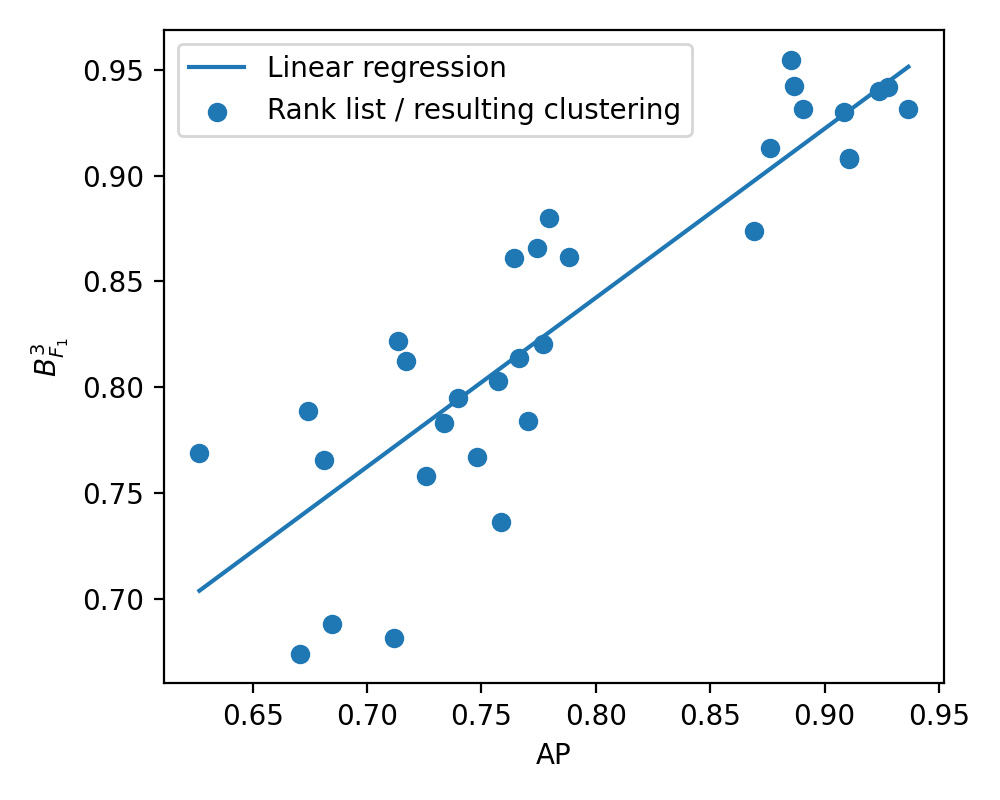
\includegraphics[width=\linewidth]{img/correlation_average_precision_b3f1_0.png}
  \subcaption{Average Linkage}
  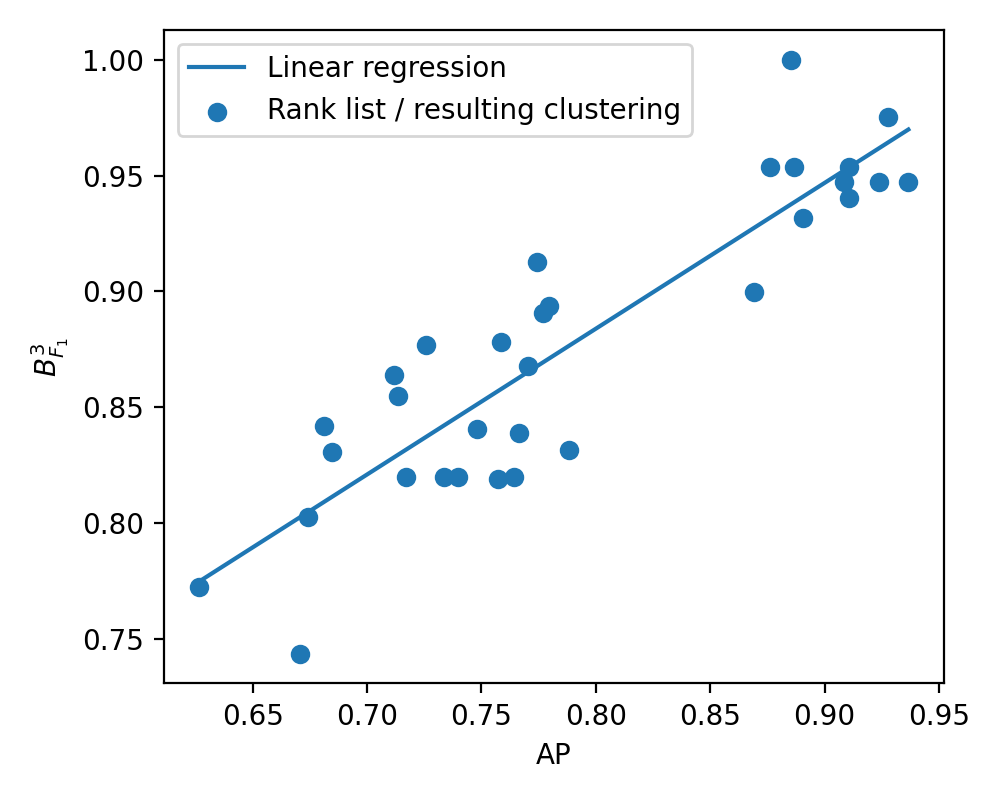
\includegraphics[width=\linewidth]{img/correlation_average_precision_b3f1_1.png}
  \subcaption{Complete Linkage}
  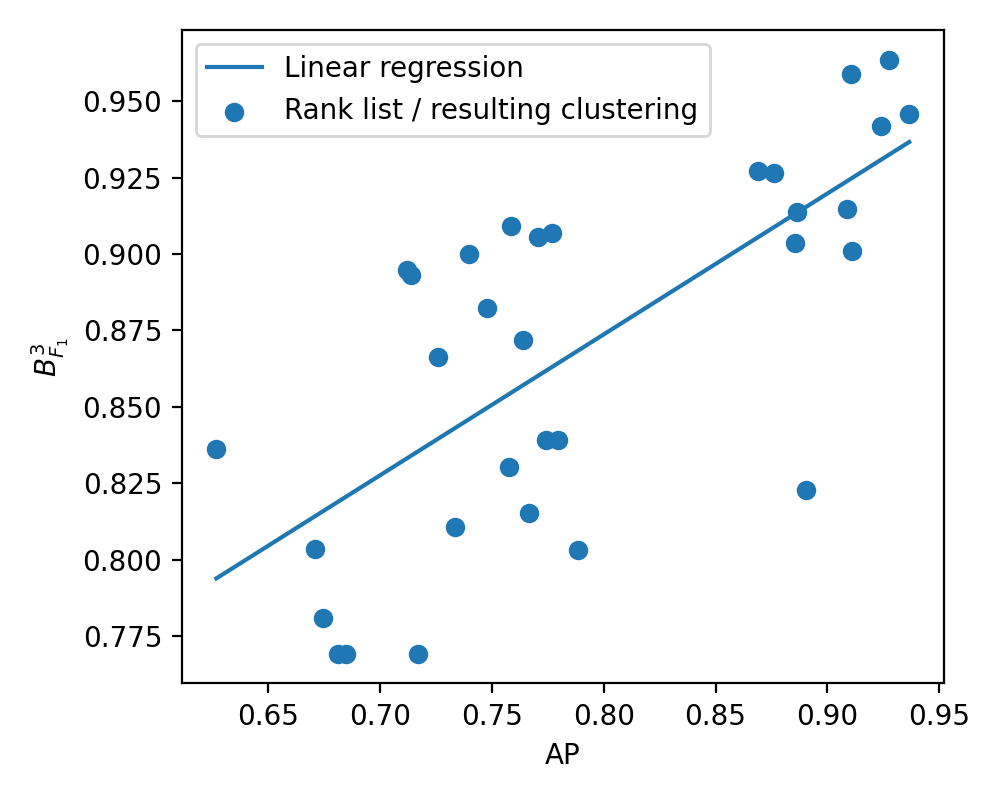
\includegraphics[width=\linewidth]{img/correlation_average_precision_b3f1_2.png}
\end{figure}
